\documentclass[10pt]{article} % For LaTeX2e
% \usepackage{tmlr}
% If accepted, instead use the following line for the camera-ready submission:
%\usepackage[accepted]{tmlr}
% To de-anonymize and remove mentions to TMLR (for example for posting to preprint servers), instead use the following:
\usepackage[preprint]{tmlr}

% Optional math commands from https://github.com/goodfeli/dlbook_notation.
\input{math_commands.tex}

%% ─── Essential packages for ML papers ───────────────────────────────────────
\usepackage{hyperref}
\usepackage{url}
\let\eqref\undefined % undo math_commands.tex \def\eqref so cleveref/amsmath can define it properly
\usepackage{booktabs}       % Professional-quality tables
\usepackage{multirow}       % Multi-row cells in tables
\usepackage{graphicx}       % Enhanced figure inclusion
\usepackage{subcaption}     % Sub-figures (a), (b), (c)
\usepackage{algorithm}      % Algorithm float environment
\usepackage{algpseudocode}  % Pseudocode typesetting (from algorithmicx, no \AND conflict)
\usepackage{xcolor}         % Colored text (for TODOs and highlights)
\usepackage{microtype}      % Improved typography and line breaking
\usepackage{xspace}         % Smart spacing after macros
\usepackage{enumitem}       % Better list control
\usepackage{wrapfig}        % Wrap text around figures
\usepackage{tablefootnote}  % Footnotes inside tables
\usepackage{amsthm}         % Theorem environments
\usepackage{tikz}           % Diagrams and drawings
\usepackage{pgfplots}       % Plots directly in LaTeX
\pgfplotsset{compat=1.18}
\usepackage[capitalize,noabbrev]{cleveref} % Smart cross-references (\cref, \Cref)

%% ─── Theorem environments ───────────────────────────────────────────────────
\newtheorem{theorem}{Theorem}[section]
\newtheorem{lemma}[theorem]{Lemma}
\newtheorem{proposition}[theorem]{Proposition}
\newtheorem{corollary}[theorem]{Corollary}
\newtheorem{conjecture}[theorem]{Conjecture}
\theoremstyle{definition}
\newtheorem{definition}[theorem]{Definition}
\newtheorem{example}[theorem]{Example}
\newtheorem{assumption}[theorem]{Assumption}
\theoremstyle{remark}
\newtheorem{remark}[theorem]{Remark}

%% ─── Collaboration macros ───────────────────────────────────────────────────
% Color-coded TODO comments (remove before submission)
\newcommand{\todo}[1]{\textcolor{red}{\textbf{[TODO: #1]}}}
\newcommand{\authorA}[1]{\textcolor{blue}{\textbf{[A1: #1]}}}
\newcommand{\authorB}[1]{\textcolor{orange}{\textbf{[A2: #1]}}}
\newcommand{\authorC}[1]{\textcolor{purple}{\textbf{[A3: #1]}}}
% Uncomment the following to suppress all comments for final submission:
% \renewcommand{\todo}[1]{}
% \renewcommand{\authorA}[1]{}
% \renewcommand{\authorB}[1]{}
% \renewcommand{\authorC}[1]{}

\newcommand{\fix}{\marginpar{FIX}}
\newcommand{\new}{\marginpar{NEW}}

\def\month{MM}  % Insert correct month for camera-ready version
\def\year{YYYY} % Insert correct year for camera-ready version
\def\openreview{\url{https://openreview.net/forum?id=XXXX}} % Insert correct link to OpenReview for camera-ready version


%% ─── Paper metadata ─────────────────────────────────────────────────────────

\title{Your Paper Title Here}

% Authors must not appear in the submitted version. They should be hidden
% as long as the tmlr package is used without the [accepted] or [preprint] options.
% Non-anonymous submissions will be rejected without review.

\author{\name First Author \email first@example.com \\
      \addr Department of Computer Science\\
      University Name
      \AND
      \name Second Author \email second@example.com \\
      \addr Department of Computer Science\\
      University Name}

% The \author macro works with any number of authors. Use \AND
% to separate the names and addresses of multiple authors.


\begin{document}


\maketitle

\begin{abstract}
State the problem you address and why it matters (1--2 sentences).
Describe your approach and key contributions (2--3 sentences).
Summarize your main results and their significance (1--2 sentences).
\end{abstract}

%% ═════════════════════════════════════════════════════════════════════════════
\section{Introduction}
\label{sec:intro}
%% ═════════════════════════════════════════════════════════════════════════════

% Paragraph 1: Motivate the problem and establish its importance.
Deep learning has driven remarkable progress across many domains~\citep{lecun2015deep, goodfellow2016deep}.

% Paragraph 2: Describe the limitations of existing approaches.
While the Transformer architecture~\citep{vaswani2017attention} has become ubiquitous,
and residual networks~\citep{he2016deep} remain foundational for vision tasks,
scaling these models efficiently remains an open challenge.

% Paragraph 3: Introduce your approach at a high level.
We propose a method that builds on pre-trained representations~\citep{devlin2019bert}
and is optimized using Adam~\citep{kingma2014adam}.

% Paragraph 4: Summarize your contributions as a list.
The main contributions of this work are:
\begin{itemize}[leftmargin=*, itemsep=2pt]
    \item Contribution one.
    \item Contribution two.
    \item Contribution three.
\end{itemize}

%% ═════════════════════════════════════════════════════════════════════════════
\section{Related Work}
\label{sec:related}
%% ═════════════════════════════════════════════════════════════════════════════

% Organize by topic, not chronologically. End each paragraph by
% differentiating your work from the cited line of research.

\paragraph{Topic A.}

\paragraph{Topic B.}

\paragraph{Topic C.}

%% ═════════════════════════════════════════════════════════════════════════════
\section{Background}
\label{sec:background}
%% ═════════════════════════════════════════════════════════════════════════════

% Define notation and cover prerequisite concepts the reader needs.

% ── amsthm: assumption and definition environments ──
\begin{assumption}[Smoothness]
    \label{asm:smooth}
    The loss function $\Loss(\params)$ is $L$-smooth, i.e.,
    $\norm{\nabla \Loss(\params) - \nabla \Loss(\params')} \leq L \norm{\params - \params'}$
    for all $\params, \params'$.
\end{assumption}

\begin{definition}[$\epsilon$-stationary point]
    \label{def:stationary}
    A point $\params$ is $\epsilon$-stationary if $\norm{\nabla \Loss(\params)} \leq \epsilon$.
\end{definition}

%% ═════════════════════════════════════════════════════════════════════════════
\section{Method}
\label{sec:method}
%% ═════════════════════════════════════════════════════════════════════════════

% Describe your approach in detail.

\subsection{Problem Formulation}
\label{sec:formulation}

% ── math\_commands macros: objective with \argmin, \Loss, \norm, \params, \dataset ──
Given a dataset $\dataset = \{(\mathbf{x}_i, y_i)\}_{i=1}^{N}$,
we seek parameters $\params^*$ that minimize:
\begin{equation}
    \params^* = \argmin_{\params} \frac{1}{N} \sum_{i=1}^{N} \Loss(f_{\params}(\mathbf{x}_i), y_i) + \lambda \norm{\params}^2
    \label{eq:objective}
\end{equation}

\subsection{Model Architecture}
\label{sec:architecture}

% ── tikz: architecture diagram ──
\begin{figure}[t]
\centering
\begin{tikzpicture}[
    node distance=1.2cm,
    block/.style={rectangle, draw, fill=blue!10, minimum width=2cm, minimum height=0.8cm, align=center, rounded corners=2pt},
    arrow/.style={->, >=stealth, thick}
]
    \node[block] (input) {Input\\$\mathbf{x} \in \reals^d$};
    \node[block, right of=input, xshift=1.5cm] (enc) {Encoder\\$f_\params$};
    \node[block, right of=enc, xshift=1.5cm] (latent) {Latent\\$\mathbf{z} \in \reals^k$};
    \node[block, right of=latent, xshift=1.5cm] (dec) {Decoder\\$g_\phi$};
    \node[block, right of=dec, xshift=1.5cm] (output) {Output\\$\hat{\mathbf{x}}$};
    \draw[arrow] (input) -- (enc);
    \draw[arrow] (enc) -- (latent);
    \draw[arrow] (latent) -- (dec);
    \draw[arrow] (dec) -- (output);
\end{tikzpicture}
\caption{Model architecture overview.}
\label{fig:architecture}
\end{figure}

\subsection{Training Procedure}
\label{sec:training}

% Example algorithm block:
\begin{algorithm}[t]
\caption{Training Procedure}
\label{alg:training}
\begin{algorithmic}[1]
\Require Dataset $\dataset$, learning rate $\eta$, epochs $T$
\Ensure Trained parameters $\params^*$
\State Initialize parameters $\params_0$
\For{$t = 1$ \textbf{to} $T$}
    \State Sample mini-batch $\mathcal{B} \subset \dataset$
    \State Compute loss $\Loss(\params_t; \mathcal{B})$
    \State $\params_{t+1} \leftarrow \params_t - \eta \nabla_{\params} \Loss(\params_t; \mathcal{B})$
\EndFor
\State \Return $\params_T$
\end{algorithmic}
\end{algorithm}

%% ═════════════════════════════════════════════════════════════════════════════
\section{Experiments}
\label{sec:experiments}
%% ═════════════════════════════════════════════════════════════════════════════

\subsection{Experimental Setup}
\label{sec:setup}

\paragraph{Datasets.}
% Describe datasets, sizes, splits, and preprocessing.

\paragraph{Baselines.}
% List and briefly describe baseline methods.

\paragraph{Implementation details.}
% Hyperparameters, optimizer, hardware, training time, etc.

\subsection{Main Results}
\label{sec:results}

% Example results table with booktabs:
\begin{table}[t]
\caption{Comparison with baselines on benchmark datasets. Best results are in \textbf{bold}, second-best are \underline{underlined}. All metrics are averaged over 3 runs $\pm$ standard deviation.}
\label{tab:main_results}
\begin{center}
\begin{tabular}{lccc}
\toprule
\textbf{Method} & \textbf{Dataset A} & \textbf{Dataset B} & \textbf{Dataset C} \\
\midrule
Baseline 1      & $85.2 \pm 0.3$     & $72.1 \pm 0.5$     & $91.0 \pm 0.2$     \\
Baseline 2      & $86.7 \pm 0.4$     & $73.8 \pm 0.3$     & $91.5 \pm 0.3$     \\
Baseline 3      & \underline{$87.3 \pm 0.2$}     & \underline{$75.2 \pm 0.4$}     & \underline{$92.1 \pm 0.2$}     \\
\midrule
\textbf{Ours}   & $\mathbf{89.1 \pm 0.2}$ & $\mathbf{77.5 \pm 0.3}$ & $\mathbf{93.4 \pm 0.1}$ \\
\bottomrule
\end{tabular}
\end{center}
\end{table}

% Example multi-panel figure:
\begin{figure}[t]
\centering
\begin{subfigure}[b]{0.32\linewidth}
    \centering
    \fbox{\rule[-.5cm]{0cm}{3cm}\rule{2.5cm}{0cm}}
    \caption{Result visualization A}
    \label{fig:result_a}
\end{subfigure}
\hfill
\begin{subfigure}[b]{0.32\linewidth}
    \centering
    \fbox{\rule[-.5cm]{0cm}{3cm}\rule{2.5cm}{0cm}}
    \caption{Result visualization B}
    \label{fig:result_b}
\end{subfigure}
\hfill
\begin{subfigure}[b]{0.32\linewidth}
    \centering
    \fbox{\rule[-.5cm]{0cm}{3cm}\rule{2.5cm}{0cm}}
    \caption{Result visualization C}
    \label{fig:result_c}
\end{subfigure}
\caption{Qualitative results. Replace placeholders with \texttt{\textbackslash includegraphics[width=\textbackslash linewidth]\{fig.pdf\}}.}
\label{fig:results}
\end{figure}

\subsection{Ablation Study}
\label{sec:ablation}

% Example ablation table:
\begin{table}[t]
\caption{Ablation study on Dataset A. Each row removes one component from the full model.}
\label{tab:ablation}
\begin{center}
\begin{tabular}{lcc}
\toprule
\textbf{Configuration}       & \textbf{Accuracy (\%)} & \textbf{$\Delta$} \\
\midrule
Full model                    & $\mathbf{89.1}$        & ---                \\
\quad w/o Component A         & $87.4$                 & $-1.7$             \\
\quad w/o Component B         & $88.0$                 & $-1.1$             \\
\quad w/o Component C         & $86.9$                 & $-2.2$             \\
\bottomrule
\end{tabular}
\end{center}
\end{table}

\subsection{Analysis}
\label{sec:analysis}

% ── cleveref: smart cross-references ──
As shown in \cref{tab:main_results}, our method outperforms all baselines.
The architecture is illustrated in \cref{fig:architecture}, and the training
procedure is detailed in \cref{alg:training}. The objective in \cref{eq:objective}
converges under \cref{asm:smooth}, as proven in \cref{thm:convergence}.

% ── xcolor + collaboration macros: color-coded comments ──
\todo{Add error bar analysis here.}
\authorA{Should we include per-class breakdown?}
\authorB{Yes, moved to \cref{app:results}.}

% ── multirow + tablefootnote + booktabs: advanced table ──
\begin{table}[t]
\caption{Results broken down by model size, showing that scaling improves performance.}
\label{tab:scaling}
\begin{center}
\begin{tabular}{llcc}
\toprule
\textbf{Model} & \textbf{Size} & \textbf{Acc. (\%)} & \textbf{FLOPs} \\
\midrule
\multirow{2}{*}{Ours}   & Small  & $87.2$ & $1.2 \times 10^9$ \\
                         & Large  & $\mathbf{89.1}$ & $4.8 \times 10^9$\tablefootnote{Measured on a single A100 GPU.} \\
\midrule
\multirow{2}{*}{Baseline} & Small  & $85.0$ & $1.1 \times 10^9$ \\
                           & Large  & $86.7$ & $4.5 \times 10^9$ \\
\bottomrule
\end{tabular}
\end{center}
\end{table}

% ── wrapfig: text wrapping around a figure ──
\begin{wrapfigure}{r}{0.35\linewidth}
    \centering
    \fbox{\rule[-.5cm]{0cm}{2.5cm}\rule{2cm}{0cm}}
    \caption{Scaling behavior.}
    \label{fig:scaling}
\end{wrapfigure}
We observe that performance scales log-linearly with compute budget,
consistent with neural scaling laws. As shown in \cref{fig:scaling},
increasing model size yields diminishing returns beyond $10^{10}$ FLOPs.
The floor of the batch size is $\floor{N / k}$ and the ceiling
is $\ceil{N / k}$, where $N$ is the dataset size and $k$ is the
number of workers. We note that $\hat{\params}_T \convp \params^*$ as
$T \to \infty$ under standard regularity conditions.

% ── enumitem: customized lists ──
Key findings from our scaling analysis:
\begin{enumerate}[label=(\roman*), itemsep=2pt]
    \item Performance scales as $\bigo{\log N}$ with dataset size.
    \item The computational cost is $\bigo{d^2}$ per layer.
    \item Memory usage grows linearly with sequence length.
\end{enumerate}

%% ═════════════════════════════════════════════════════════════════════════════
\section{Discussion}
\label{sec:discussion}
%% ═════════════════════════════════════════════════════════════════════════════

% Interpret results, discuss limitations, and suggest future work.

\paragraph{Limitations.}
% Be upfront about what your method does not handle well.

\paragraph{Future work.}
% Concrete next steps, not vague aspirations.

%% ═════════════════════════════════════════════════════════════════════════════
\section{Conclusion}
\label{sec:conclusion}
%% ═════════════════════════════════════════════════════════════════════════════

% Restate the problem, your solution, and the key takeaway (3--5 sentences).

\subsubsection*{Broader Impact Statement}
In this optional section, TMLR encourages authors to discuss possible repercussions of their work,
notably any potential negative impact that a user of this research should be aware of.
Authors should consult the TMLR Ethics Guidelines available on the TMLR website
for guidance on how to approach this subject.

\subsubsection*{Reproducibility Statement}
% Describe what you have done to ensure reproducibility:
% code availability, hyperparameter tables, random seeds, etc.

\subsubsection*{Author Contributions}
If you'd like to, you may include a section for author contributions as is done
in many journals. This is optional and at the discretion of the authors. Only add
this information once your submission is accepted and deanonymized.

\subsubsection*{Acknowledgments}
Use unnumbered third level headings for the acknowledgments. All
acknowledgments, including those to funding agencies, go at the end of the paper.
Only add this information once your submission is accepted and deanonymized.

\bibliography{main}
\bibliographystyle{tmlr}

\appendix

\section{Additional Experimental Results}
\label{app:results}
% Full tables, per-class breakdowns, additional visualizations.

\section{Theoretical Results}
\label{app:proofs}
% Detailed proofs that are too long for the main text.

% ── amsthm + cleveref: theorem with cross-reference ──
\begin{theorem}[Convergence rate]
    \label{thm:convergence}
    Under \cref{asm:smooth}, SGD with step size $\eta = 1/L$ satisfies:
    \begin{equation}
        \frac{1}{T} \sum_{t=0}^{T-1} \expect{\norm{\nabla \Loss(\params_t)}^2}
        \leq \frac{2L \left( \Loss(\params_0) - \Loss^* \right)}{T} + \frac{\sigma^2}{T}
    \end{equation}
    where $\Loss^* = \inf_\params \Loss(\params)$ and $\sigma^2$ is the variance of the stochastic gradient.
\end{theorem}

\begin{proof}
    By $L$-smoothness of $\Loss$ we have \ldots
\end{proof}

\section{Implementation Details}
\label{app:implementation}
% Full hyperparameter tables, architecture diagrams, training curves.

% ── pgfplots: training curve ──
\begin{figure}[h]
\centering
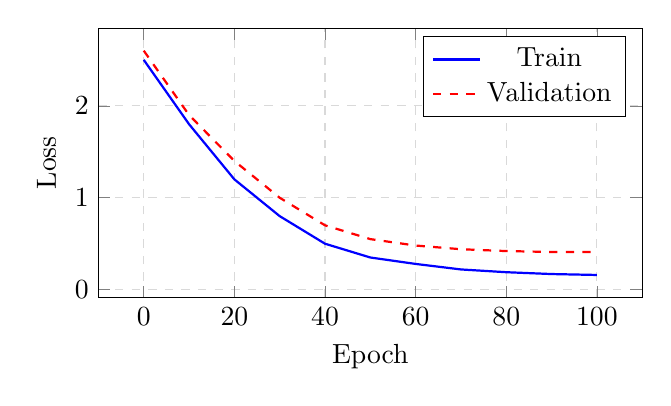
\begin{tikzpicture}
\begin{axis}[
    width=0.7\linewidth,
    height=5cm,
    xlabel={Epoch},
    ylabel={Loss},
    legend pos=north east,
    grid=major,
    grid style={dashed, gray!30},
]
\addplot[blue, thick] coordinates {(0,2.5)(10,1.8)(20,1.2)(30,0.8)(40,0.5)(50,0.35)(60,0.28)(70,0.22)(80,0.19)(90,0.17)(100,0.16)};
\addlegendentry{Train}
\addplot[red, thick, dashed] coordinates {(0,2.6)(10,1.9)(20,1.4)(30,1.0)(40,0.7)(50,0.55)(60,0.48)(70,0.44)(80,0.42)(90,0.41)(100,0.41)};
\addlegendentry{Validation}
\end{axis}
\end{tikzpicture}
\caption{Training and validation loss curves.}
\label{fig:training_curves}
\end{figure}

% Example hyperparameter table:
\begin{table}[h]
\caption{Hyperparameters used in all experiments.}
\label{tab:hyperparams}
\begin{center}
\begin{tabular}{lc}
\toprule
\textbf{Hyperparameter}   & \textbf{Value} \\
\midrule
Learning rate              & $3 \times 10^{-4}$ \\
Batch size                 & 256 \\
Weight decay               & $10^{-5}$ \\
Optimizer                  & AdamW \\
LR schedule                & Cosine annealing \\
Warmup steps               & 1000 \\
Training epochs            & 100 \\
Hidden dimension           & 768 \\
Number of layers           & 12 \\
Attention heads            & 12 \\
Dropout                    & 0.1 \\
\bottomrule
\end{tabular}
\end{center}
\end{table}

\end{document}
